\chapter{Design}
For the purpose of the successful completion of this project I have decided to employ agile software development methodologies with evolutionary prototyping. The reason for taking this approach are the strengths of the agile software developmental methodology which is that it is incremental, cooperative, flexible and adaptive \cite{4147390}. Our project is addressing an issue which does not have well specified set of requirements and the clients do not have a clear view of what they actually expect. This led us to use  evolutionary prototyping \cite{Connell89} as this helps minimise the impact of misunderstanding or miscommunication of the requirements. The risk of which are relatively high as the goals of this project are relatively new and there is not much similar work done. This technique would also give better idea of what the end product would be capable of and would look like to the client. With evolutionary prototyping the system is continuously refined and improved. Each iteration builds on top of the previous thus meaning that with each increment we add more functionality and features or/and refine/improve what has already been implemented. Simply stated, this means that with each iteration we are one step closer to the end product. This allows us to add features which were not previously considered or remove ones that are no longer viable or needed. In addition, this approach allows us to engage with the key stakeholders very early in the project life-cycle. This will provide us with valuable feedback which again brings a lot of advantages:

\begin{itemize}
	\item The delivery of the tool is speeded up and also minimises the risks of failing to deliver a working product before the project deadline \cite{Connell89}.
	\item Users would engage with the product early in the project lifetime. This however, poses some risk like the users requesting more features which were not previously mentioned or discussed. This means that we need to maintain some balance as this project has a fixed deadline and limited resources.
	\item Increased chances of fully understanding and meeting the user requirements and expectations from the tool.
\end{itemize}

Each increment (iteration) consists of the following stages:
\begin{enumerate}
	\item Requirements specification \& refinement
	\item Design
	\item Prototype implementation \& Testing
	\item User testing and feedback provision
	\item Evaluate
\end{enumerate}
The requirements and specification step would document what the tool should look and work like at the end of each iteration. These would be following the aims and objectives we have defined in Chapter 1 of this report. After a prototype has been implemented and tested by the user, we will evaluate the progress and make any changes in out requirements, design and project plan accordingly. Thus after a number of iterations, we should have a prototype which to resemble the desired product as required by the user.

In the below sections I have presented the system at an abstract level. This follows from careful analysis and consideration of the requirements stated in the previous chapter. I have tried to highlight all major key components and classes which are described formally. This allows us to better organise and structure our problem. The diagrams presented follow the unified modelling language (UML) paradigm \cite{uml} and are platform-independent models (PIM) of the system. This allows us to focus on the design of the system itself without distracting our attention with platform specific decisions. Once these models are created we can than easily transform them into platform specific models (PSM) using the desired technologies.
%This technique is known as Model-Driven Architecture (MDA) software design approach \cite{mda}.

\section{Use cases}
Based on the user requirements stated in the previous chapter, a use case diagram has been derived and presented in figure~\ref{fig:useCase} below. The use case diagram depicts the way users (actors) interact with the tool (system). There are three types of users of the system (every next type is extension of the previous as it can be seen from the diagram):
\begin{itemize}
	\item \textbf{Normal} users are people with general access to the system. They have read-only right and can interact with the system by requesting a list of disruptions and more details for a selected from them disruption. They also have access to the disruption history of the network. This use case was not in the initial requirements and was identified as a useful feature during demonstrations of the prototype to TFL.
	\item \textbf{Operator} is assumed to be a CentreComm staff member who is required to authenticate into the system. This would allow them the extra functionalities of adding comments to disruptions for others to see. Such users also have the functionality of hiding and showing disruptions that are currently detected in the bus network available to them.
	\item \textbf{Administrator} users have the most privileges of all type of users of the system. In addition to the above actions they are also allowed to view and change the configuration settings of the system. This is to allow easier configuration of the application.
\end{itemize}

\begin{figure}
	\makebox[\textwidth][c]{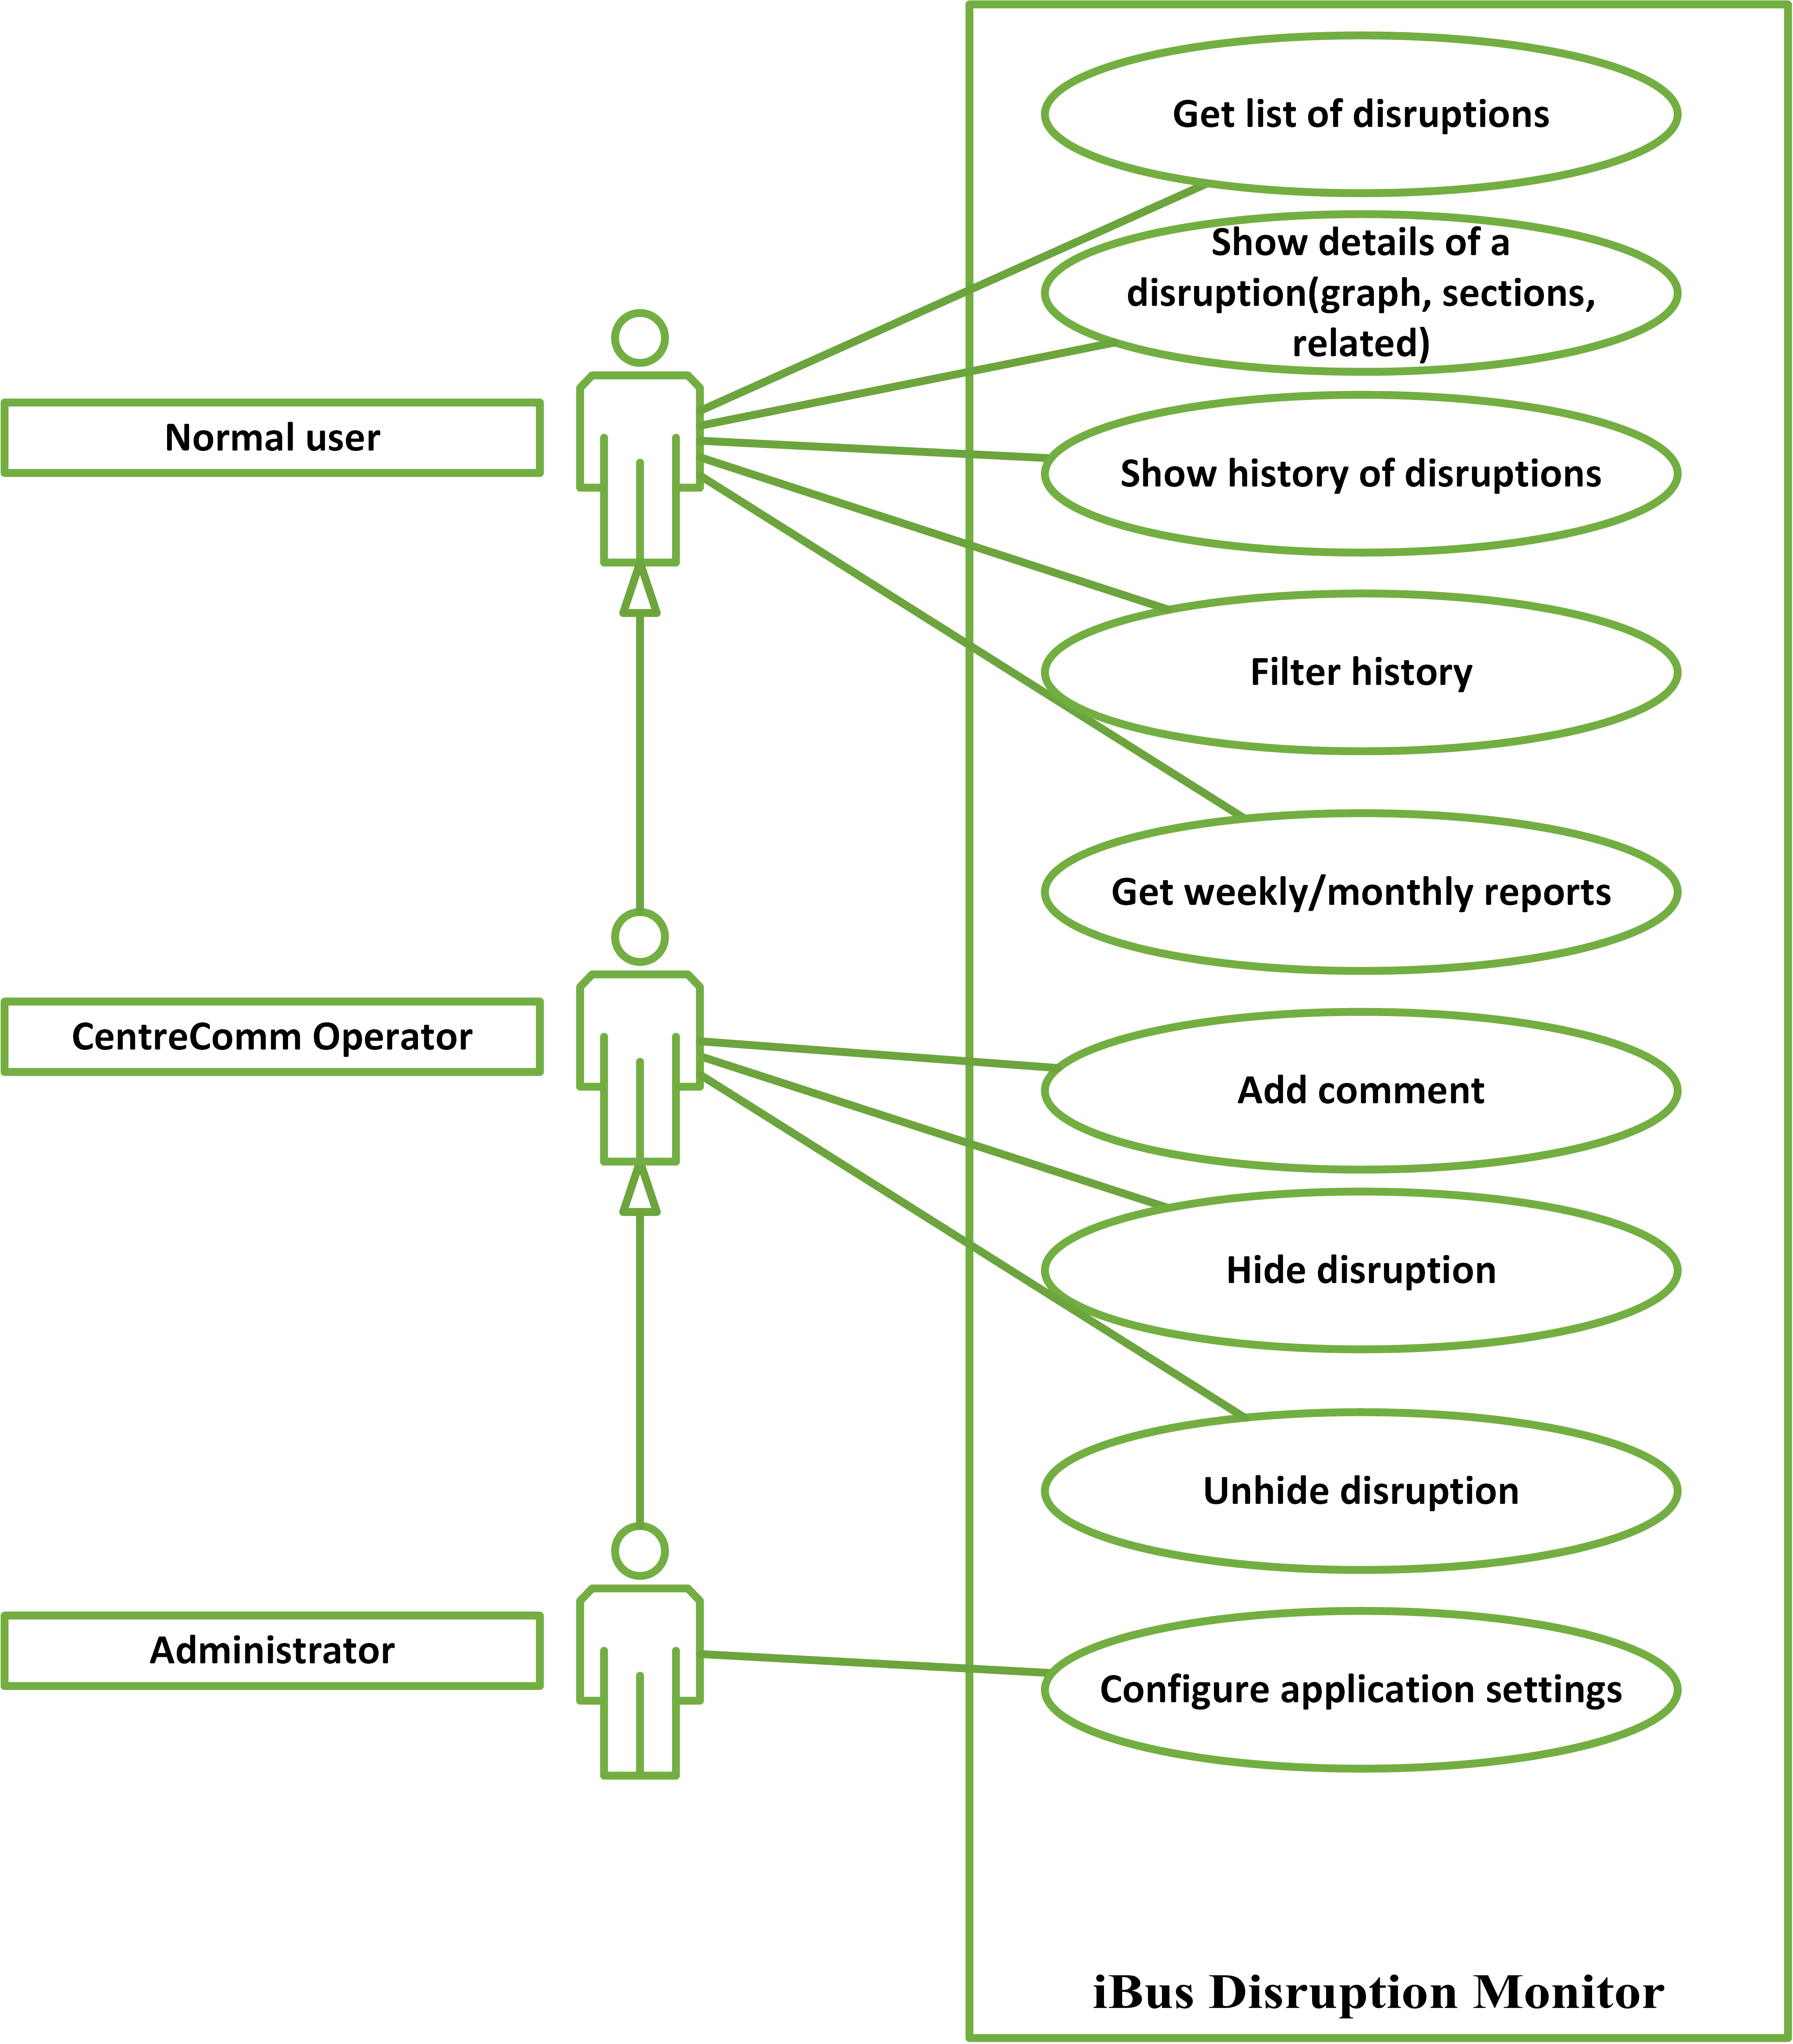
\includegraphics[width=1.2\textwidth]{Figures/UseCases.png}}
	\caption{Use Case Diagram}
\label{fig:useCase}
\end{figure}

\FloatBarrier
\section{System architecture}
In figure~\ref{fig:systemArchitecture} the architecture diagram of the system could be seen. The overall architecture is following a four-tier architecture with a model view controller (MVC) pattern for the user interface. This architecture allows us to decompose to system into separate subsystems where lower tiers do not depend on higher tiers. This system allows for the implementation details of subsystems to be changed without affecting other components if the interfaces do not change.

As it can be seen from the diagram the system is divided in four main layers:
\begin{itemize}
	\item \textbf{Representation Layer} - It consists of a number of user views and is responsible for visualisation of the user interface. 
	\item \textbf{Representation  Control Layer} - responsible for the control/transition between user interface windows. In this layer I have made use of the front controller pattern \cite{fowler2003patterns} as it allows us to combine the common logic in one controller.
	\item \textbf{Application Logic Layer} -  this layer is the functional core of the system. This is where all the business logic is encoded and corresponding calculations are done. The most important part of the system is the Disruption Engine which is responsible for:
	\begin{enumerate}
		\item Monitoring for new feeds and processing them.
		\item Updating the bus network status (calculating delays and detecting disruptions).
		\item Writing the changes to the system database.
	\end{enumerate}
	The Disruption Model is the other major component of the system. It is responsible for retrieving the disruptions and their details from the database and providing them to the representation control tier.
	\item \textbf{Data Layer} - this is the data repository layer responsible for storing and maintaining the underlying system data. It consists of comma separated values (CSV) files representing the AVL feeds that are being pushed to the system. Here we also have the system database which contains all the configuration settings parameters and the output of the engine (disruptions and their details that are detected by the tool).
\end{itemize}
This architecture diagram in figure~\ref{fig:systemArchitecture} represents coarse grained view of the system to be implemented. Each of the components presented above could be implemented as a number of smaller components and modules depending on the specific technologies.

\begin{figure}
	\makebox[\textwidth][c]{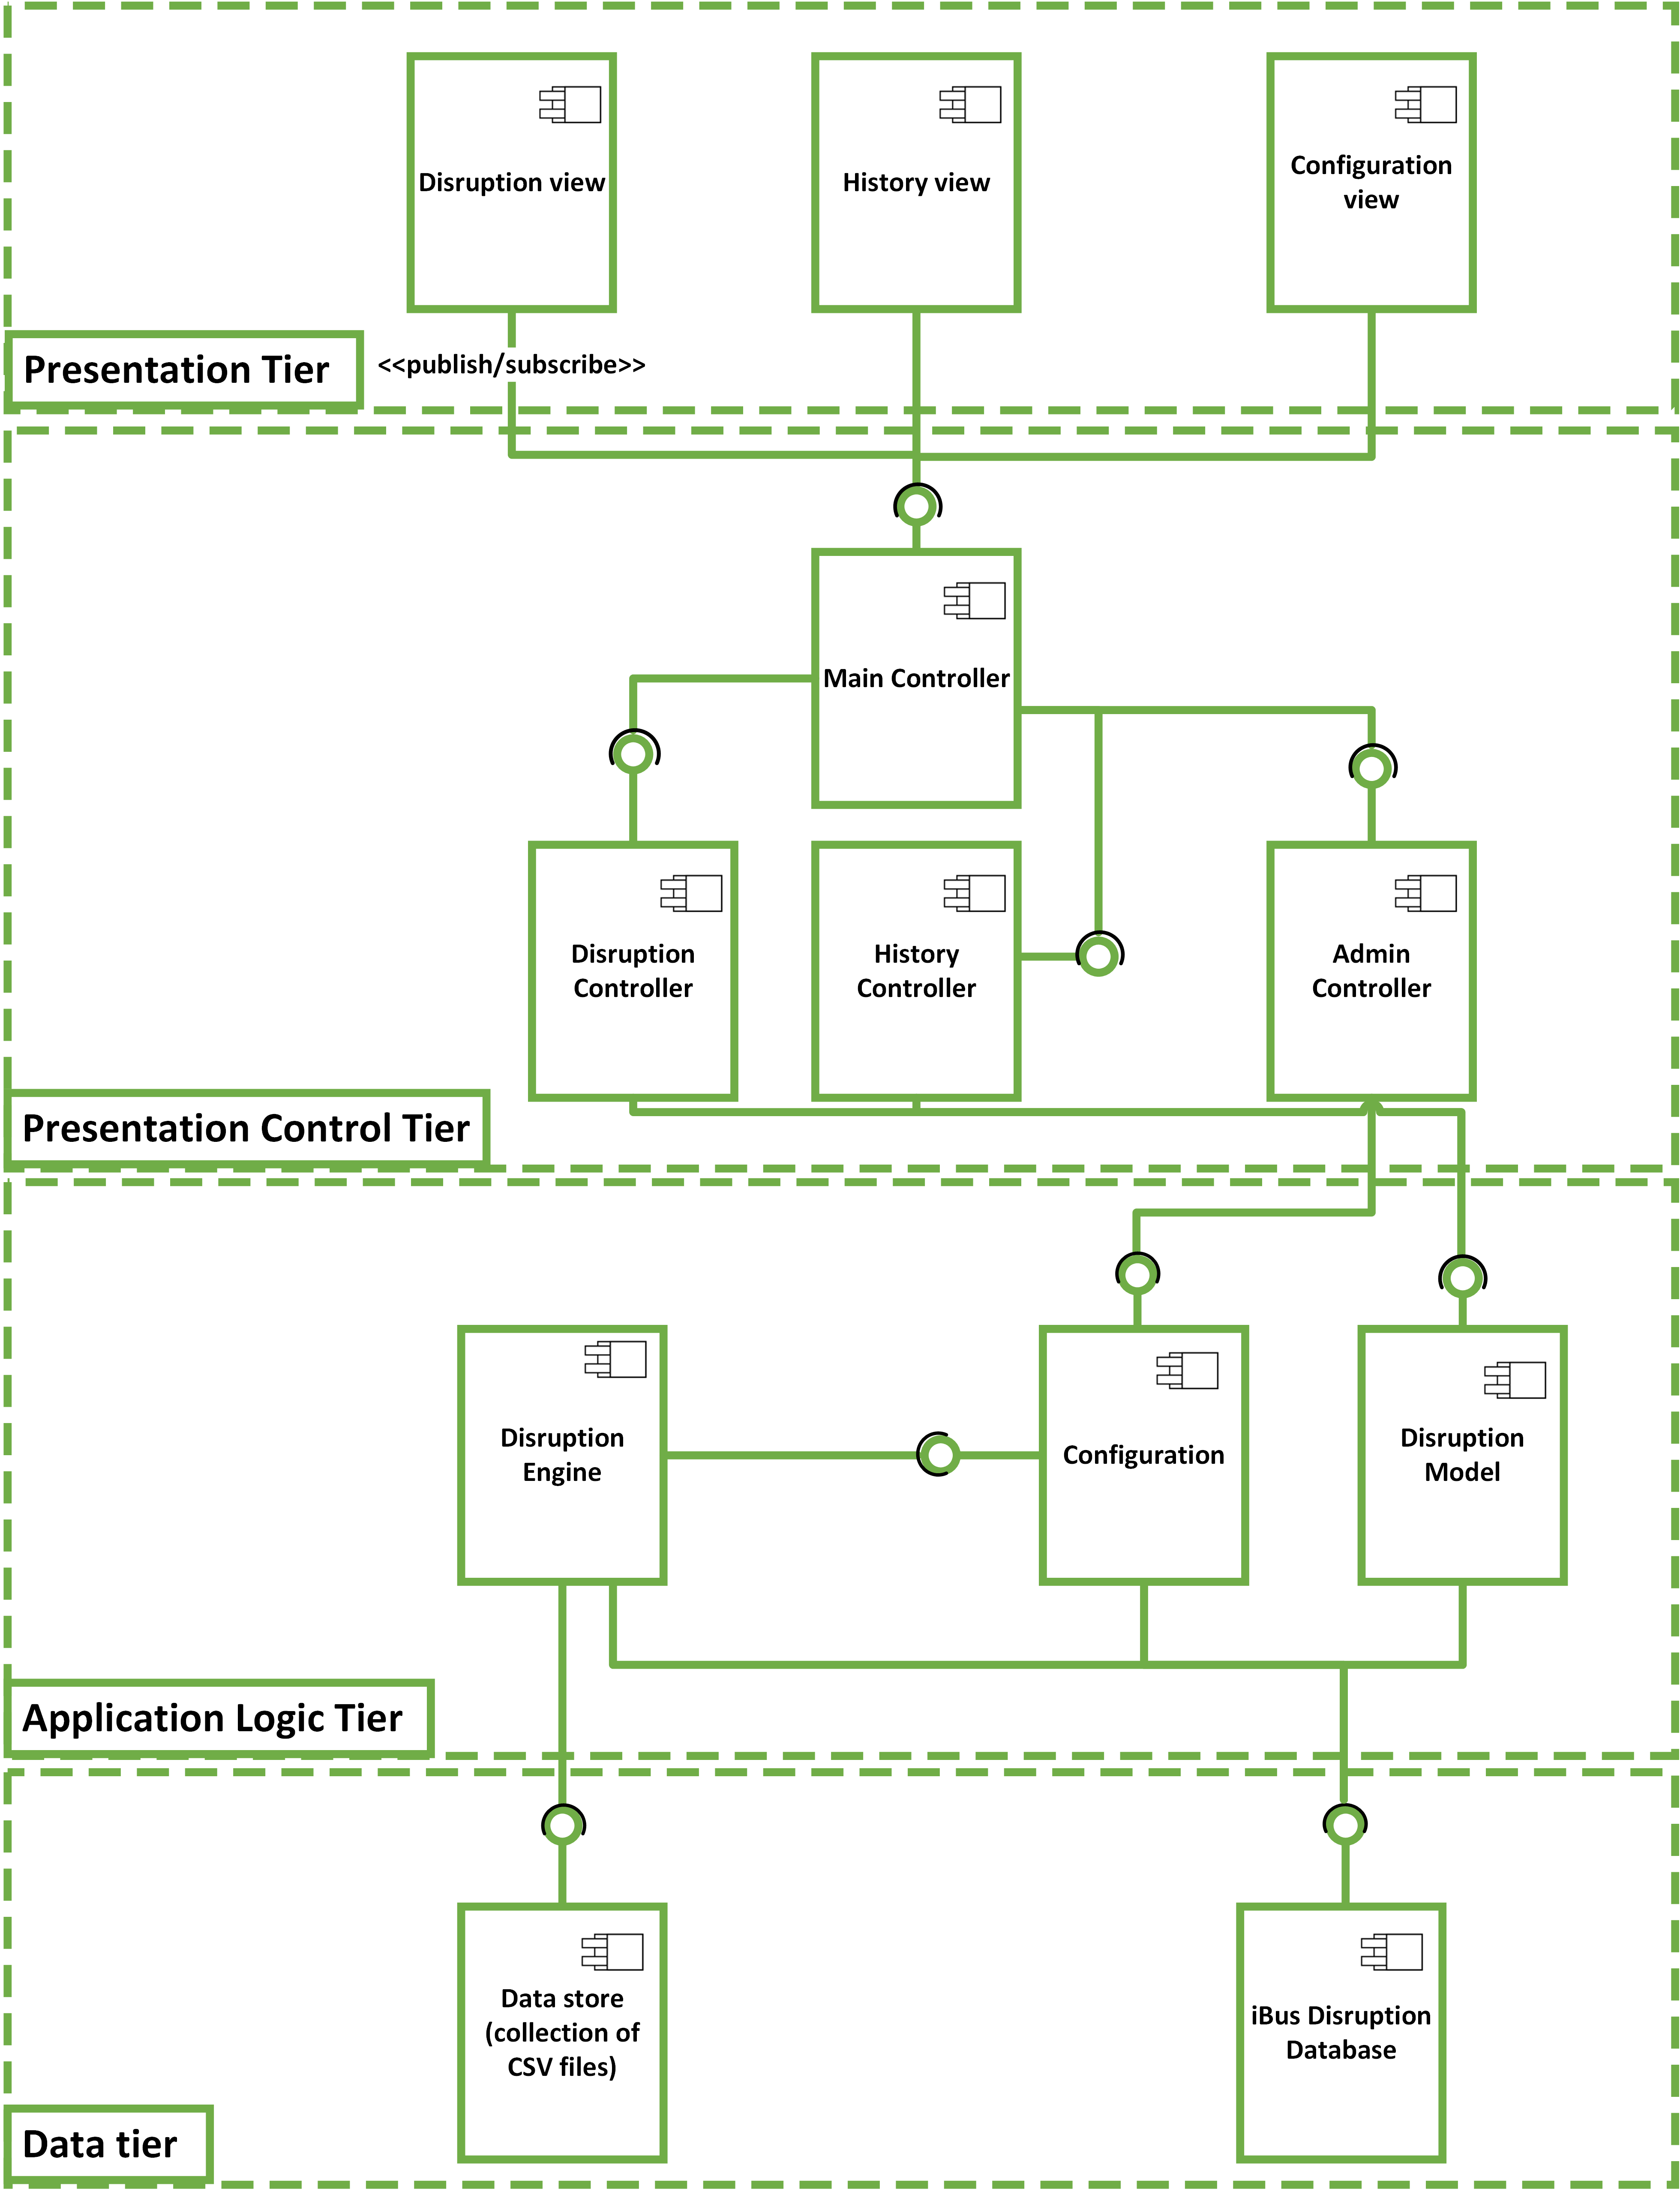
\includegraphics[width=1.2\textwidth]{Figures/Architecture.png}}
	\caption{System Architecture Diagram}
\label{fig:systemArchitecture}
\end{figure}

\FloatBarrier
\section{State Machine}
State machine diagrams are useful in explaining in what states the system could reside and how it transitions from one state to the other. The state machine diagram of the disruption engine component of our system is presented in figure~\ref{fig:stateMachine} below. This diagram represents the states in which the disruption engine could reside and the available transitions. As it can be seen from the figure, once the engine is initialised correctly it enters a continuous loop. This loop represents the engine waiting for new feeds to be detected by the system. Once detected they are processed and the bus network state is updated. If this update results in no changes in the state of the bus network compared to the previous observed state, the tool does not make any changes to the database, else it would write all the changes that have been detected and calculated. In case the system fails to connect or write the changes to the database the system terminates producing the appropriate error alerting the maintenance personnel. This behaviour is appropriate for this project as its scope is to produce a proof concept working prototype rather than a fully functional ready to deploy production tool.

\begin{figure}
	\makebox[\textwidth][c]{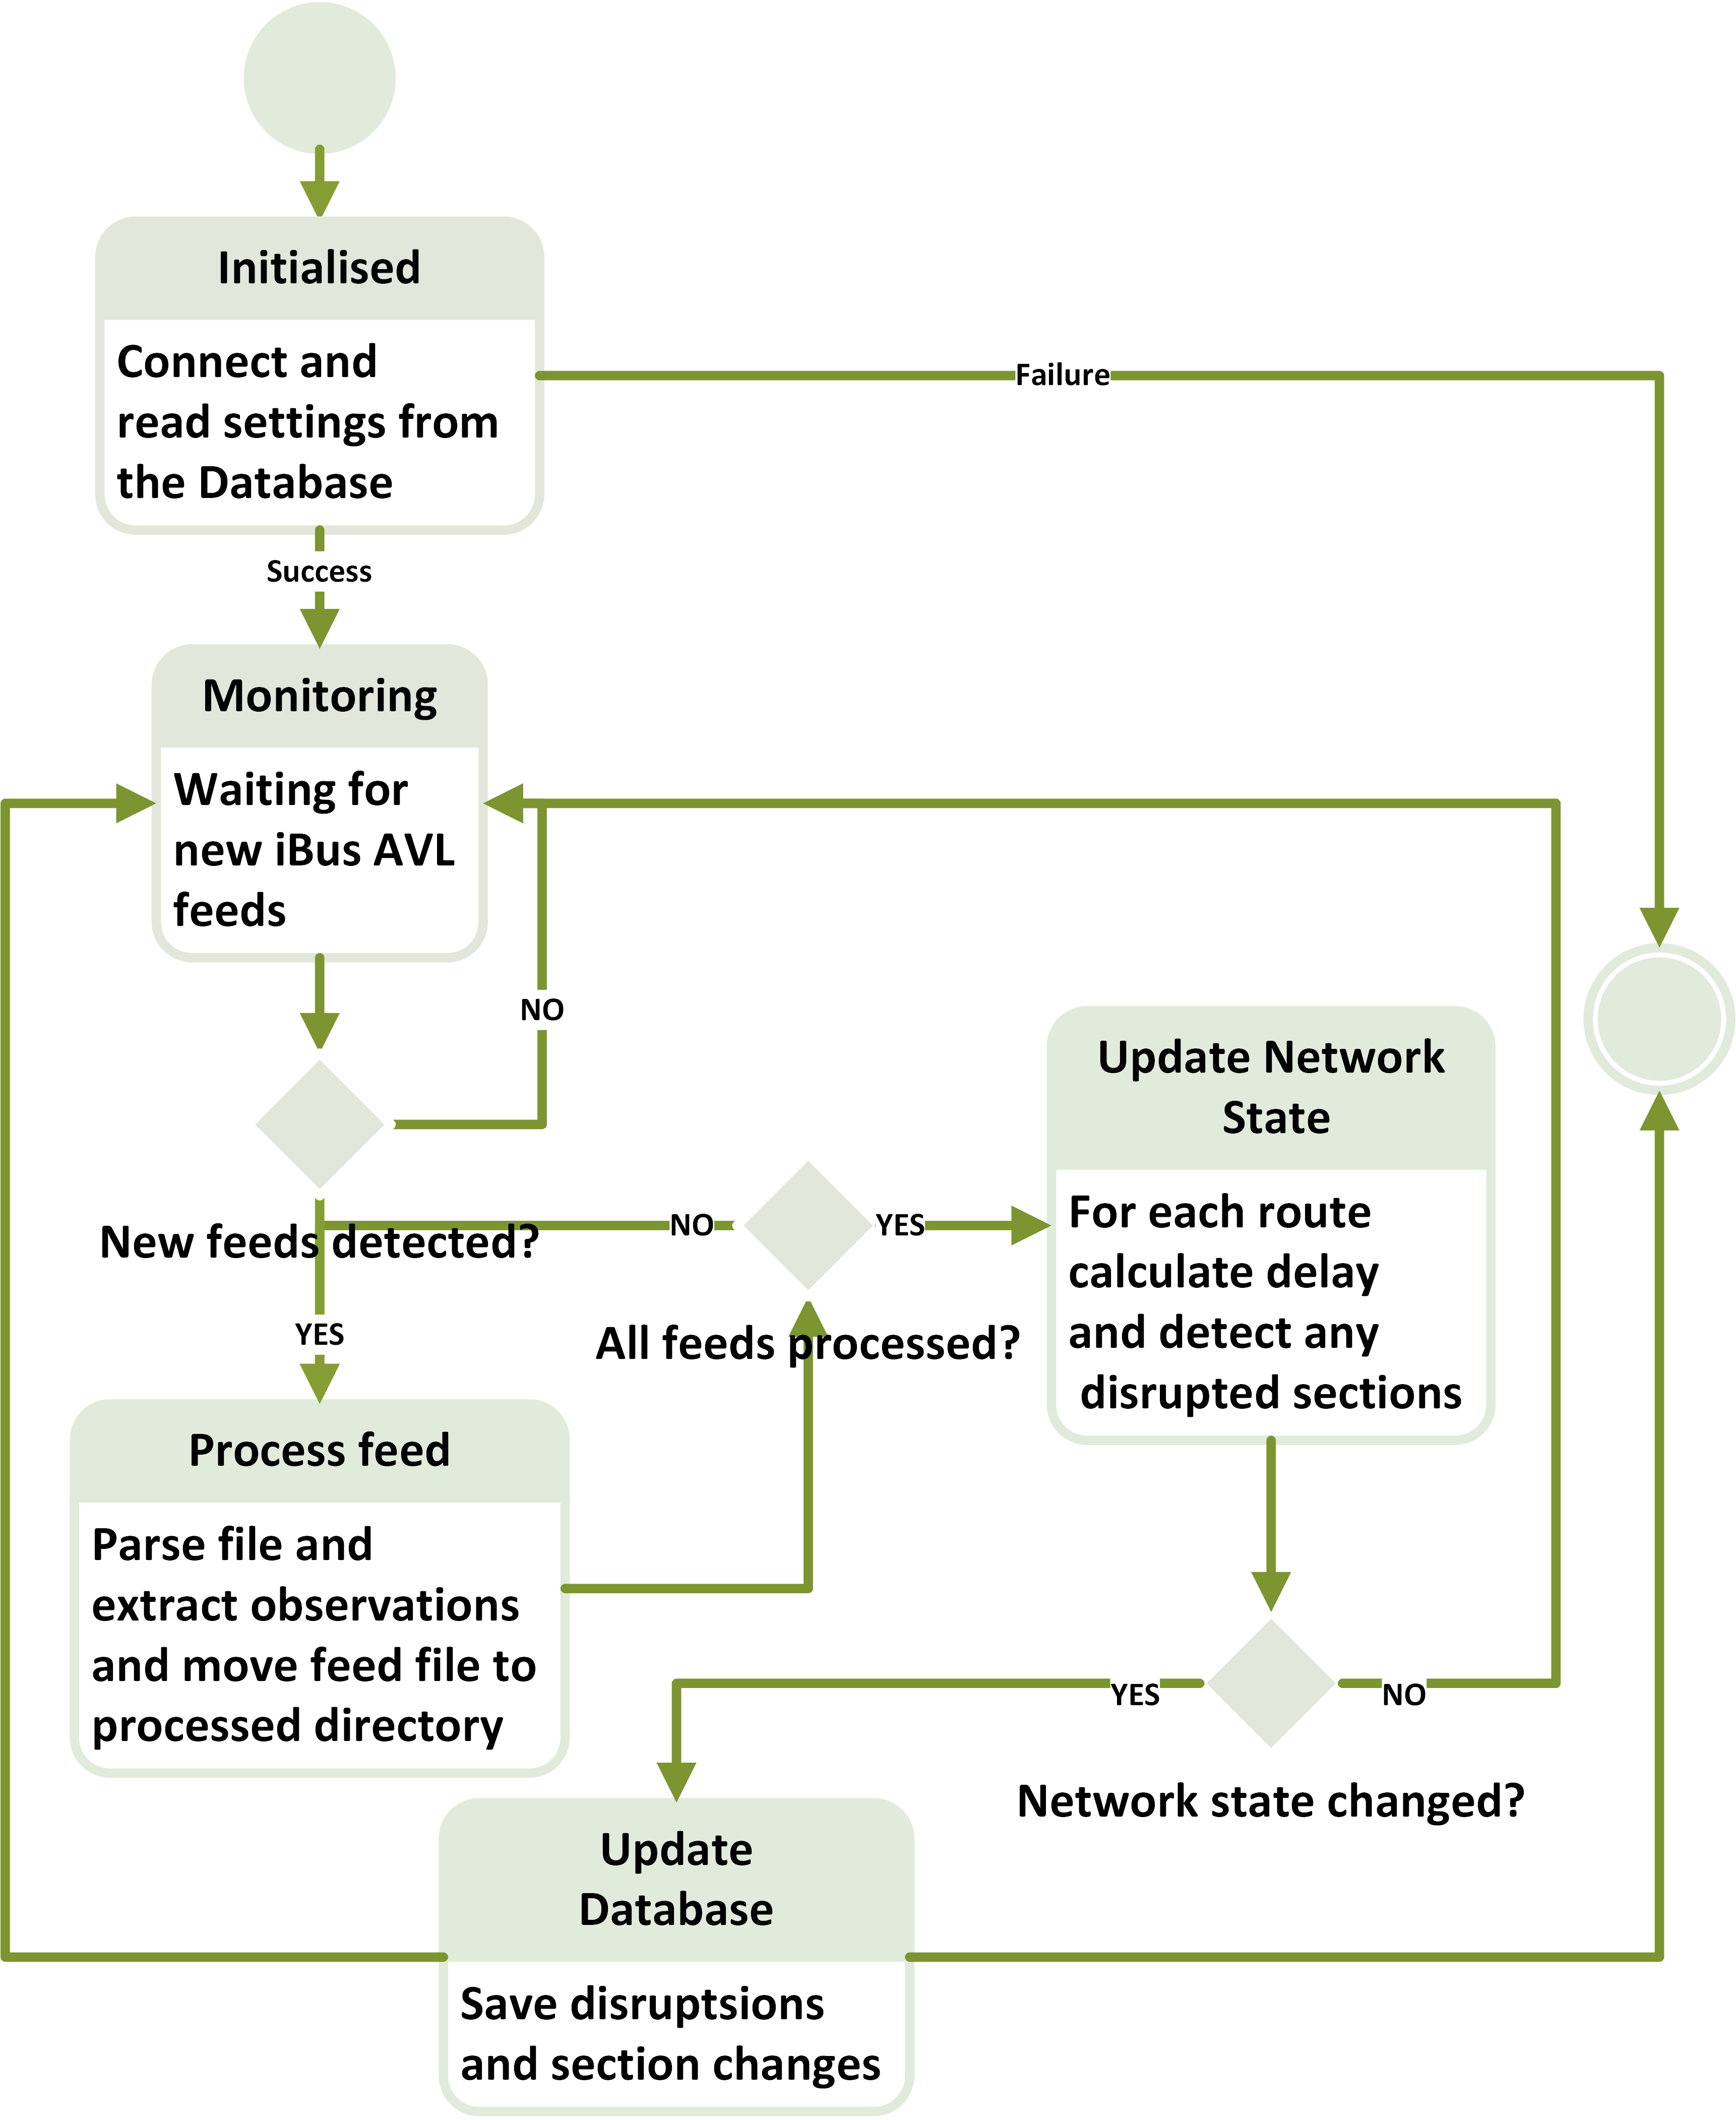
\includegraphics[width=1.2\textwidth]{Figures/StateDiagram.png}}
	\caption{State Machine Diagram}
\label{fig:stateMachine}
\end{figure}

\FloatBarrier
\section{Class organisation}
Class decomposition diagrams are the main building block of object oriented programming paradigm. They are widely used tool for the organisation and design of a software system. The diagram consist of classes, which encapsulate some attributes (state) and methods (functionalities), and the associations between the individual class. Each class is depicted by a box with the name of the class on top and its member attributes and methods below. Associations are represented by lines connecting those classes where a relation exists. In figure~\ref{fig:useCase} below we have depicted the class diagram of the disruption engine component from the architecture diagram. We have only presented the class diagram of this component as this is the component which captures the main business logic with regards to detecting the disruptions in the bus network. In the following subsections I have provided some explanation of the most important classes in the class diagram.

\subsection{iBusMonitor}
This could be viewed as the entry point of the tool engine. The most notable and important attribute of the iBusMonitor class is the link to the configuration file specifying the database connection properties. It can have a number of bus networks and is responsible for initialising the tool and monitoring. This means it encapsulates the logic for listening for new feed files being published.

\subsection{BusStop}
The bus stop class is representation of a bus stop in the bus network. It consists of a number of expected attributes that a stop would have. We also make the assumption that a single stop can belong to only one bus network.

\subsection{BusNetwork}
This class represent a given bus network. In the context of this project this can be viewed as the TFL bus network. This object encapsulates all attributes that relate to the network state and its behaviour. Each bus network consists of at least one bus stop and at least one route otherwise it does not make any sense to have a network without any stops or routes.

\subsection{Route}
This class is one of the most important in the context of this project as it encapsulates the state of a single route in the network. Each route is associated with at least one run (in most cases each route would have two runs In/Out-bound) and a number of observations. 

\subsection{Run}
This object represent a route's run state and methods. Its main properties consist of list of consecutive readings made on this run for each logged bus. It also provides interface for detecting and updating disruptions on this run, thus it needs to keep track of the disruptions that were previously seen along this run.

\subsection{Section}
This is the most basic part of a bus route, apart from the bus stop. Each section represents the part of the route between two consecutive bus stops along this route. This means it is characterised by a start and end stop and the sequence of this section along the route. In this class we calculate the delay per individual section (more on how this is done in the following chapter).

\subsection{Observation}
The observation class captures the state and functionality of a single observation. By observation we mean a single reading extracted from the AVL data input. This reading is expected to be coming from a single bus logged on a given bus route, thus it would belong to this route. 

\subsection{Disruption}
This class simply captures all the attributes of a disruption. Each disruption would have an identification number, sections between the disruption is observed and the corresponding delay and trend. It also provides methods for updating and saving the details to the database.

\begin{figure}
	\makebox[\textwidth][c]{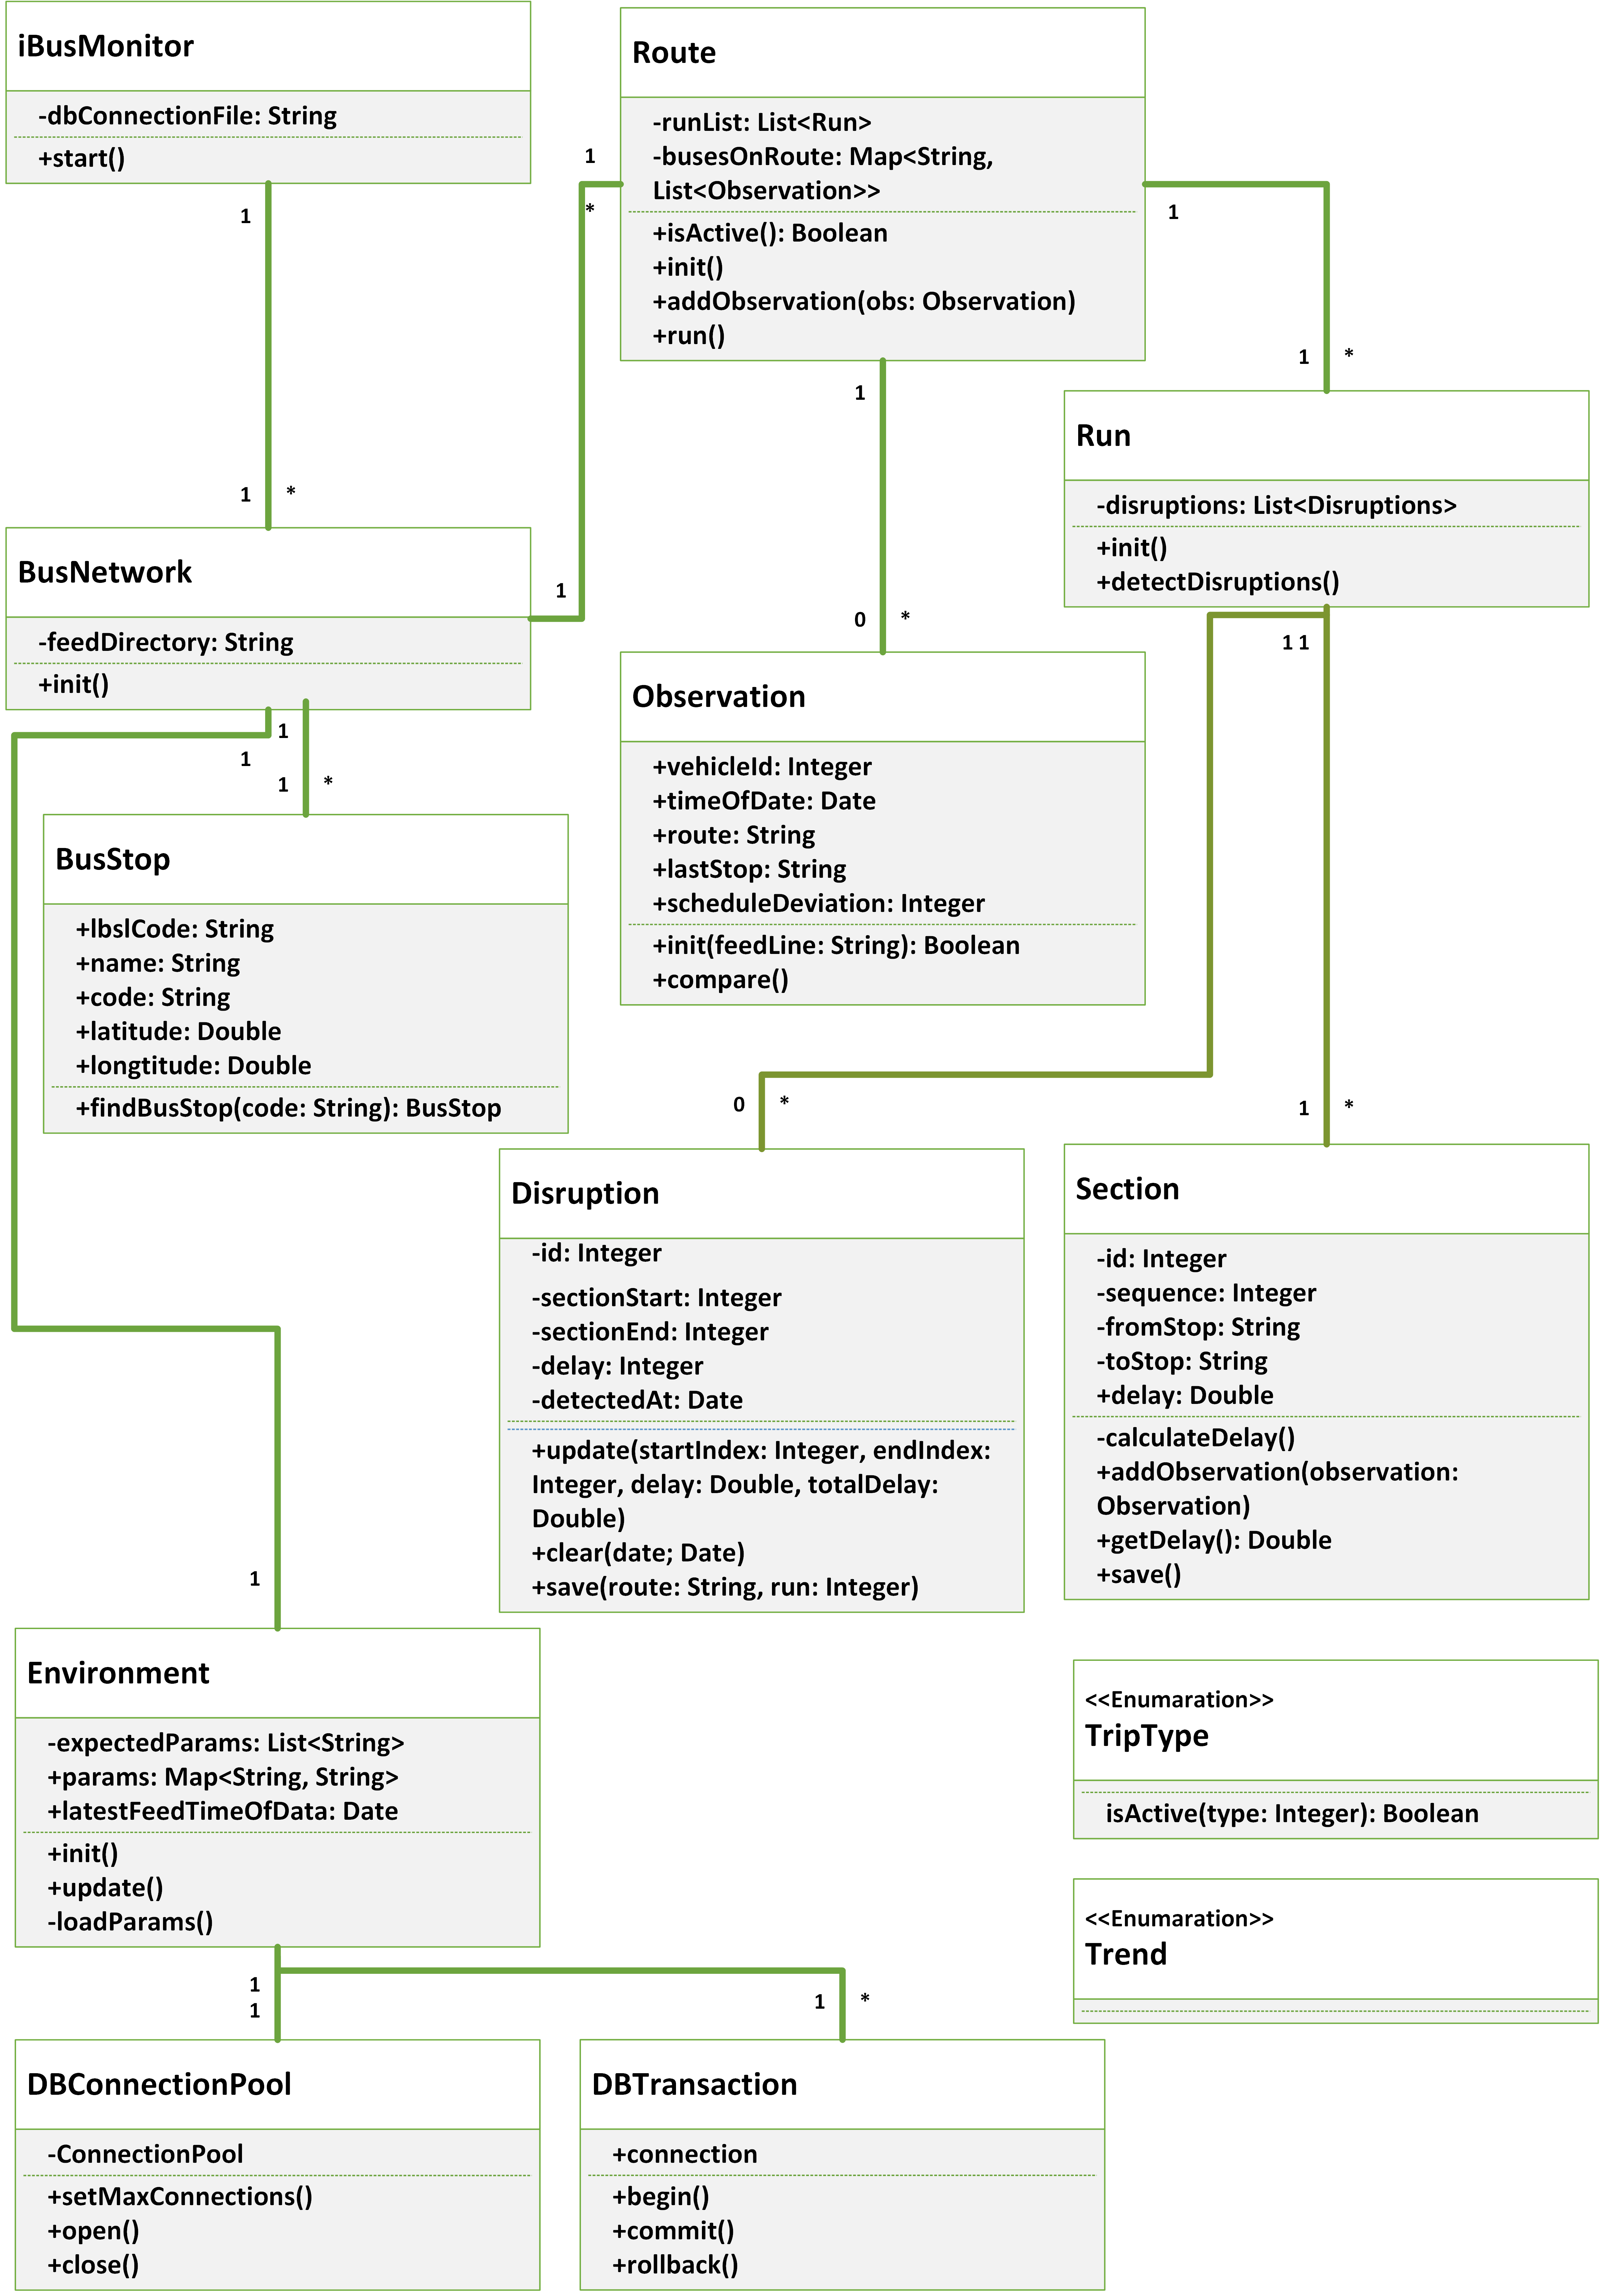
\includegraphics[width=1.2\textwidth]{Figures/Class.png}}
	\caption{Class Diagram}
\label{fig:class}
\end{figure}

\FloatBarrier
\section{User Interface}
The user interface of our system is addressing the second main aim of this project the one of visualising the calculated list of delays. The design and rational behind the user interface has been developed throughout discussions and meetings with CentreComm staff. The main requirement for the design is to be easy to identify the most important issues in the network. One of the uses of the user interface would be on a large monitoring multi-screen video walls which to be used not only by CentreComm, but by Traffic Management and even the Metropolitan Police. Another usage would be by the individual operators to access it through their personal computers. 

The above use cases and requirements have led to the decision of using a web-based application for the purpose of satisfying them fully. Using web rather than a standalone application, we allow for our system to be accessible from any device capable of running a browser (e.g. computer, laptop, smart TV, smart-phone, tablet etc.). Another advantage is that we only need to deploy the web application once and it can be universally accessed through the local network or even through the internet.

In order to improve separations of concerns we have also decided to have separate application for the disruption engine and the user interface. This means that we can change each one without affecting the other (considering we maintain the correct interfaces). This also allows us to implement and add more user interfaces apart from the web application if needed. For example we may even latter want to create a dedicated mobile (tablet or smart-phone) application using the output from the disruption engine. This separation also allows to have different dedicated specialised people for maintaining each of the applications.

We have decided to use tabular approach for visualising the prioritised list of disruption. Each entry in the list would give detail of the route and section which are delayed. It also provides the time when the disruption was first detected. Any additional information is only provided on request from the user.

The overall architecture of the structure of the user interface can be seen in the architecture diagram in figure A.2 in Appendix A. An early mock-up of the graphic user interface can be seen in figure~\ref{fig:guiProposal}. This has however evolved a lot throughout the project. In Chapter 5 below we will give detailed description of the implemented visualisation and show the end user interface.


\begin{figure}[ht]
	\makebox[\textwidth][c]{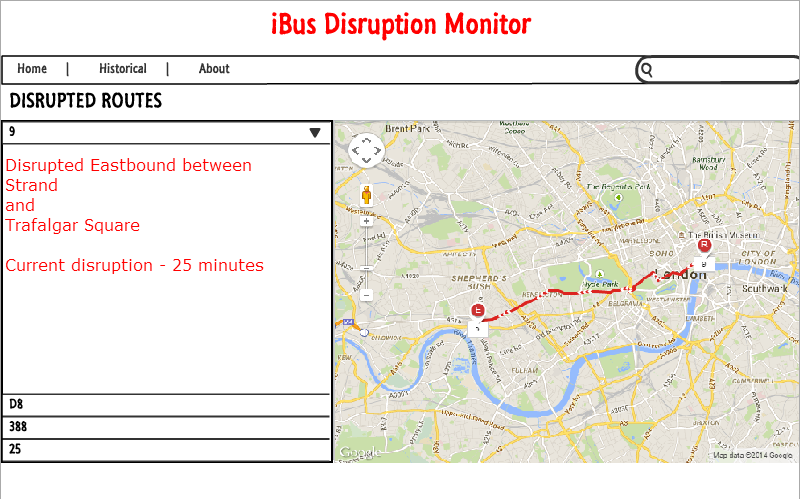
\includegraphics[width=1\textwidth]{Figures/guiProposal.png}}
	\caption{Initial GUI mock-up}
	\label{fig:guiProposal}
\end{figure}